\chapter[Problema 02]{Problema 02}

\section{Mensagens Utilizando Ping}

O ping é uma ferramenta útil para testar conectividade da rede entre equipamentos, ele utiliza o protocolo ICMP para enviar e receber mensagens. Dois tipos de mensagens são utilizadas: 

\begin{itemize}
	\item O tipo 8 que corresponde a um comando "ECHO request", emitido pela máquina fonte; 
	\item O tipo 0 que corresponde a um comando "ECHO reply", emitido pelo maquina alcançada; 
\end{itemize}



O host escolhido para realização dessa atividade foi o www.harvard.edu cujo endereço de IP é 54.240.160.86. 

Primeiramente o servidor de DNS foi consultado para que fosse possível ter acesso ao IP associado ao domínio informado, tendo conhecimento do mesmo, fez-se uso do protocolo ICMP enviando uma mensagem to tipo "Echo request" que pode ser observado na Figura \ref{fig:ping}. Em resposta ao pacote de número 60 o pacote de numéro 61 enviou uma mensagem "Echo reply".


  \begin{figure}[h]
    \centering

    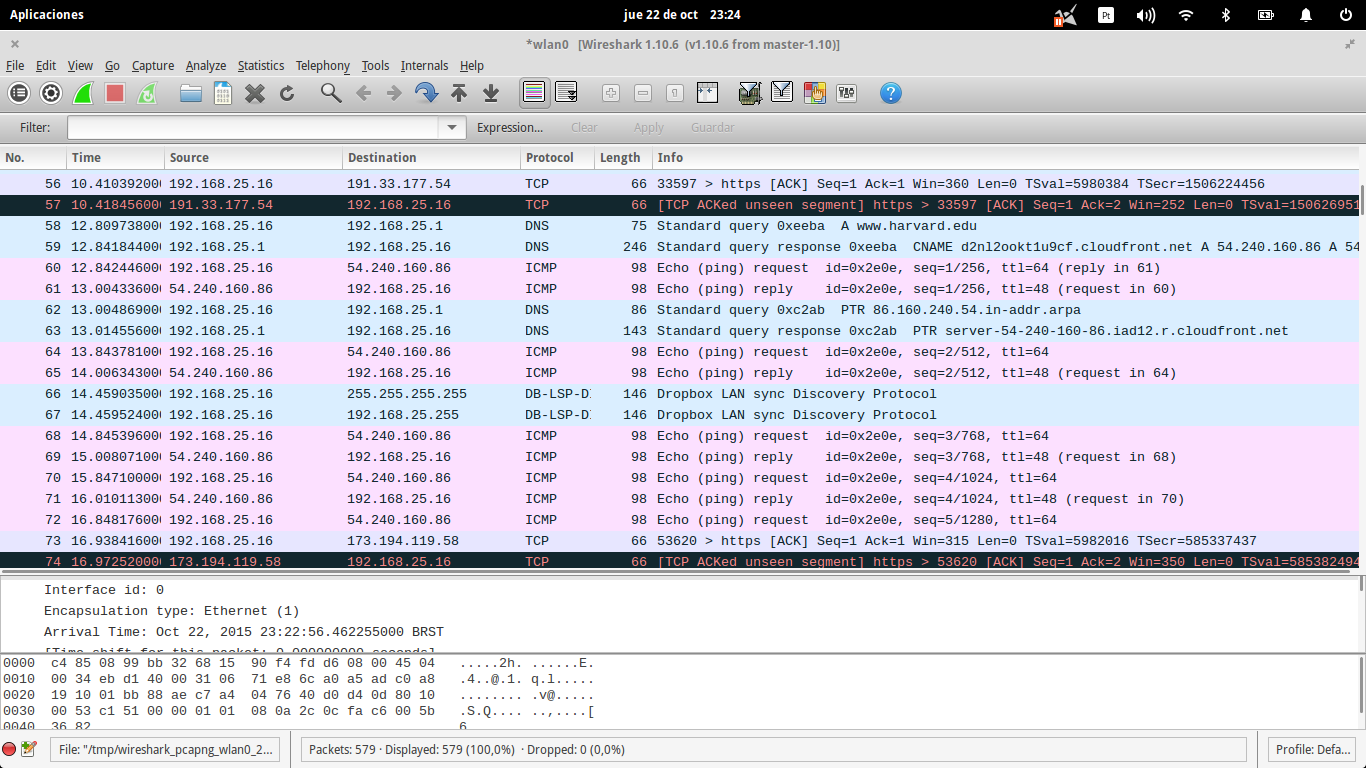
\includegraphics[width=450px, scale=1]{figuras/ping}
    \caption{Capturas de Pacotes em uma transação PING}

 \label{fig:http}
  \end{figure}

% The typical process is:

% You enter a command to ping a destination.

% DNS is used to determine the IP address (if needed).

% The routing table is consulted to find the next hop towards that destination.

% ARP is used to find the hardware address of the next hop.

% The IP packet is sent to the next hop, encapsulated in an Ethernet or WiFi frame.


% O ping funciona da seguinte maneira:
% -- indicar evolução nas capturas.


\section{Mensagens Utilizando Nmap}
\section{Mensagens Utilizando Traceroute}
